\documentclass[a4paper, oneside, 12pt, english]{article}
\usepackage{geometry}
\geometry{
	a4paper,
	total={154mm,232mm},
	left=28mm,
	top=32mm,
}
\setlength{\parskip}{0.85em}
\setlength{\parindent}{2.6em}
\usepackage{array}
\usepackage{amsmath}
\usepackage{amssymb}
\usepackage{enumerate}
\usepackage{graphicx}
\usepackage{url}
\usepackage{color}
\usepackage{wrapfig}
\usepackage{systeme}
\usepackage{tabularx}
\usepackage{subfig}
\usepackage{hyperref}
\usepackage[authoryear, round]{natbib}
\usepackage[dvipsnames]{xcolor}

\newcommand{\rw}{\color{red}\textbf{?} \color{black}}		% When something needs to be reworded

\begin{document}
\begin{titlepage}
	\newcommand{\HRule}{\rule{\linewidth}{0.5mm}}
	\center
	\textsc{\LARGE Université de Liège}\\[1cm]
	\textsc{\Large Faculté des Sciences Appliquées}\\[2cm]
		
	\HRule \\[0.5cm]
	{ \huge \bfseries Automatic Multispeaker Voice Cloning}\\[0.2cm]
	\HRule \\[2cm]

	\begin{minipage}{0.4\textwidth}
		\begin{flushleft} \Large
			\emph{Author:}\\
			Corentin \textsc{Jemine}
		\end{flushleft}
	\end{minipage}
	~
	\begin{minipage}{0.4\textwidth}
		\begin{flushright} \Large
			\emph{Supervisor:} \\
			Prof. Gilles \textsc{Louppe}
		\end{flushright}
	\end{minipage}\\[4cm]
	
	{\LARGE Academic year 2018 - 2019}\\[1cm]
	
	
\includegraphics{images/uliege_logo.jpg}\\[1.25cm]
	
	\textit{Graduation studies conducted for obtaining the Master's degree \\in Data Science by Corentin Jemine}
	
	\vfill
\end{titlepage}
\setcounter{page}{2}

%\color{red}
%Possibly, start with a TTS lexicon with some definitions. Meanwhile, I'll make a list of TTS-specific words that may be worth explaining:\\
%coarticulation\\
%linguistic context\\
%spectral envelope\\
%fundamental frequency\\
%contour (a way in which something varies especially the pitch of music or the pattern of tones in an utterance.)\\
%supra-segmental\\
%grapheme
%\color{black}
%\clearpage

\section*{Abstract}
Recent advances in deep learning have shown impressive results in the domain of text-to-speech. To this end, a deep neural network is usually trained using a corpus of several hours of professionally recorded speech from a single speaker. Giving a new voice to such a model is highly expensive, as it requires recording a new dataset and retraining the model. A recent research introduced a three-stage pipeline that allows to clone a voice unseen during training from only a few seconds of reference speech, and without retraining the model. The authors share remarkably natural-sounding results, but provide no implementation. We reproduce this framework and open-source the first public implementation of it. We adapt the framework with a newer vocoder model, so as to make it run in real-time.
\clearpage

\tableofcontents
\clearpage

\section{Introduction}
% What is now possible with deep learning in TTS
Deep learning models have become predominant in many fields of applied machine learning. text-to-speech (TTS), the process of synthesizing artificial speech from a text prompt, is no exception. Deep models that would produce more natural-sounding speech than the traditional concatenative approaches begun appearing in 2016. Much of the research focus has been since gathered around making these deep models more efficient, more natural, or training them in an end-to-end fashion. Inference has come from being hundreds of times slower than real-time on GPU \citep{WaveNet} to possible in real-time on a mobile CPU \citep{WaveRNN}. As for the quality of the generated speech, \citet{Tacotron2} demonstrate near human naturalness. Interestingly, speech naturalness is best rated with subjective metrics; and comparison with actual human speech leads to the conclusion that there might be such a thing as "speech more natural than human speech". In fact, some argue that the human naturalness threshold has already been crossed \citep{MOSNaturalness}.

% The state of things in TTS
Datasets of professionally recorded speech are a scarce resource. Synthesizing a natural voice with a correct pronunciation, lively intonation and a minimum of background noise requires training data with the same qualities. Furthermore, data efficiency often remains one of the shortcomings of deep learning. Training a common text-to-speech model such as Tacotron \citep{Tacotron1} typically requires tens of hours of speech. %It is thus no surprise that there seems to be a theme in speech-related applications of reproducing the voice of whomever is the current president of the United States. %-> kinda funny but not necessary
Yet the ability of generating speech with any voice is attractive for a range of applications be they useful or merely a matter of customization. Research has led to frameworks for voice conversion and voice cloning. They differ in that voice conversion is a form of style transfer on a speech segment from a voice to another, whereas voice cloning consists in capturing the voice of a speaker to perform text-to-speech on arbitrary inputs. 

% What voice cloning is about
While the complete training of a single-speaker TTS model is technically a form of voice cloning, the interest rather lies in creating a fixed model that is able to incorporate newer voices with little data. The common approach is to condition a TTS model trained to generalize to new speakers on an embedding of the voice to clone~\citep{DeepVoice2, CloningFewSamples, SV2TTS}. The embedding is low-dimensional and derived by a speaker encoder model that takes reference speech as input. This approach is typically more data efficient than training a separate TTS model for each speaker, in addition to being orders of magnitude faster and less computationally expensive. Interestingly, there is a large discrepancy between the duration of reference speech needed to clone a voice among the different methods, ranging from half an hour per speaker to only a few seconds.

% What we want to achieve
Our objective is to achieve a powerful form of voice cloning. The resulting framework must be able to operate in a zero-shot setting, that is, for speakers unseen during training. It should incorporate a speaker's voice with only a few seconds of reference speech. These desired results are shown to be fulfilled by \citep{SV2TTS}. Their results are impressive\footnote{\url{https://google.github.io/tacotron/publications/speaker_adaptation/index.html}}, but not backed by any public implementation. We reproduce their framework and make our implementation open-source\footnote{\color{red} repo link}. In addition, we integrate the model of \citep{WaveRNN} in the framework to make it run in real-time, i.e. to generate speech in a time shorter or equal to the duration of the produced speech. \color{red} add a word about our results \color{black}

% Structure of the thesis
The structure of this document goes as follows. We begin with a short introduction on TTS methods that involve machine learning. Follows a review of the evolution of the state of the art for TTS and for voice cloning. We then present the work of \citep{SV2TTS} as is, without mention of our own implementation. The remainder of this document focuses on the three individual parts of the framework, and on our implementation of the whole.


\section{A review of text-to-speech methods in machine learning}
\subsection{Statistical parametric speech synthesis}
% The SPSS pipeline
Statistical parametric speech synthesis (SPSS) refers to a group of data-driven TTS methods that emerged in the late 90s. In SPSS, the relationship between the features computed on the input text and the output acoustic features is learned by a statistical generative model (called the acoustic model). A complete SPSS framework thus also includes a pipeline to extract features from the text to synthesize, as well as a system able to reconstruct an audio waveform from the acoustic features produced by the acoustic model (such a system is called a vocoder). Unlike the acoustic model, these two parts of the framework may be entirely engineered and make use of no statistical methods. While modern deep TTS models are usually not referred to as SPSS, the SPSS pipeline as depicted in figure \ref{spss_framework} applies just as well to those newer methods.

\begin{figure}[h]
	\centering
	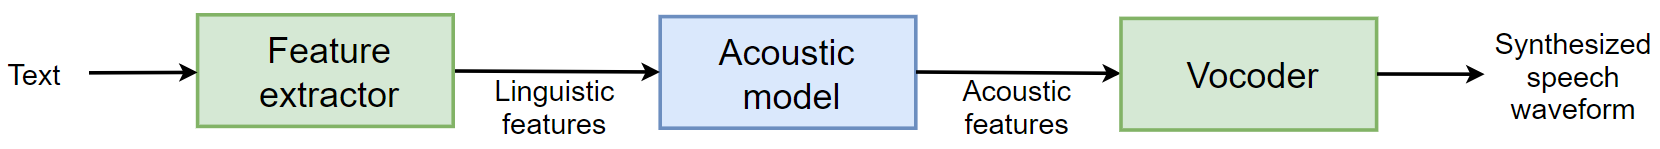
\includegraphics[width=\linewidth]{images/spss_framework.png}
	\caption{The general SPSS pipeline. The blue box is purely a statistical model while the green boxes can be engineered processes or/and statistical models.}
	\label{spss_framework}
\end{figure}

% Purpose of the feature extractor
The role of the feature extractor is to provide data that is more indicative of what the speech produced by the model is expected to sound like. Speech is a complex process, and directly feeding characters to a weak acoustic model will prove not to be effective. Providing additional features from natural language processing (NLP) techniques may greatly reduce the extent of the task to be learned by the acoustic model. It may however result in trade-offs when it comes to naturalness, especially for rare or unknown words. Indeed, manually engineered heuristics do not quite fully characterize all intricacies of spoken language. For this reason, feature extraction can also be done with trained models. The line between the feature extractor and the acoustic model can then become blurry, especially for deep models. In fact, a tendency that is common across all areas where deep models have overtaken traditional machine learning techniques is for feature extraction to consist of less heuristics, as models become able to operate at higher levels of abstraction.

% Feature extraction techniques
A common feature extraction technique is to build frames that will integrate surrounding context in a hierarchical fashion. For example, a frame at the syllable level could include the word that comprises it, its position in the word, the neighbouring syllables, the phonemes that make up the syllable, ... The lexical stress and accent of individual syllables can be predicted by a statistical model such as a decision tree. To encode prosody, a set of rules such as ToBI \citep{TOBI} can be used. Ultimately, there remains a work of feature engineering to present a frame as a numerical object to the model, e.g. categorical features are typically encoded using a one-hot representation.

% Spectrogram vs waveform
One could wonder why the acoustic model does not directly predict an audio waveform. Audio happens to be difficult to model: it is a particularly dense domain and audio signals are typically highly nonlinear. A representation that brings out features in a more tractable manner is the time-frequency domain. Spectrograms are much less dense than their waveform counterpart and also have the benefit of being two-dimensional, thus allowing models to better leverage spatial connectivity. Unfortunately, a spectrogram is a lossy representation of the waveform that discards the phase. There is no unique inverse transformation function, and deriving one that produces natural-sounding results is not trivial. When referring to speech, this generative function is called a vocoder. The choice of the vocoder is an important factor in determining the quality of the generated audio.

\color{red}Talk about evaluation metrics (MOS and A/B testing)?\color{black}


\subsection{Evolution of the state of the art in text-to-speech}
The state of the art in SPSS has for long remained a hidden Markov model (HMM) based framework \citep{Tokuda-2013}. This approach, laid out in figure \ref{hmm_spss_framework}, consists in clustering the linguistic features extracted from the input text with a decision tree, and to train a HMM per cluster \citep{HMMTTS}. The HMMs are tasked to produce a distribution over spectrogram coefficients, their derivative, second derivative and a binary flag that indicates which parts of the generated audio should contain voice. With the maximum likelihood parameter generation algorithm (MLPG) \citep{Tokuda-2000}, spectrogram coefficients are sampled from this distribution and eventually fed to the MLSA vocoder \citep{MLSA}. It is possible to modify the voice generated by conditioning the HMMs on a speaker or tuning the generated speech parameters with adaptation or interpolation techniques \citep{HMMSpeakerInterpolation}. Note that, while this framework used to be state of the art for SPSS, it was still inferior in terms of the naturalness of the generated speech compared to the well-established concatenative approaches.

\begin{figure}[h]
	\centering
	\begin{minipage}{.45\linewidth}
		\centering
		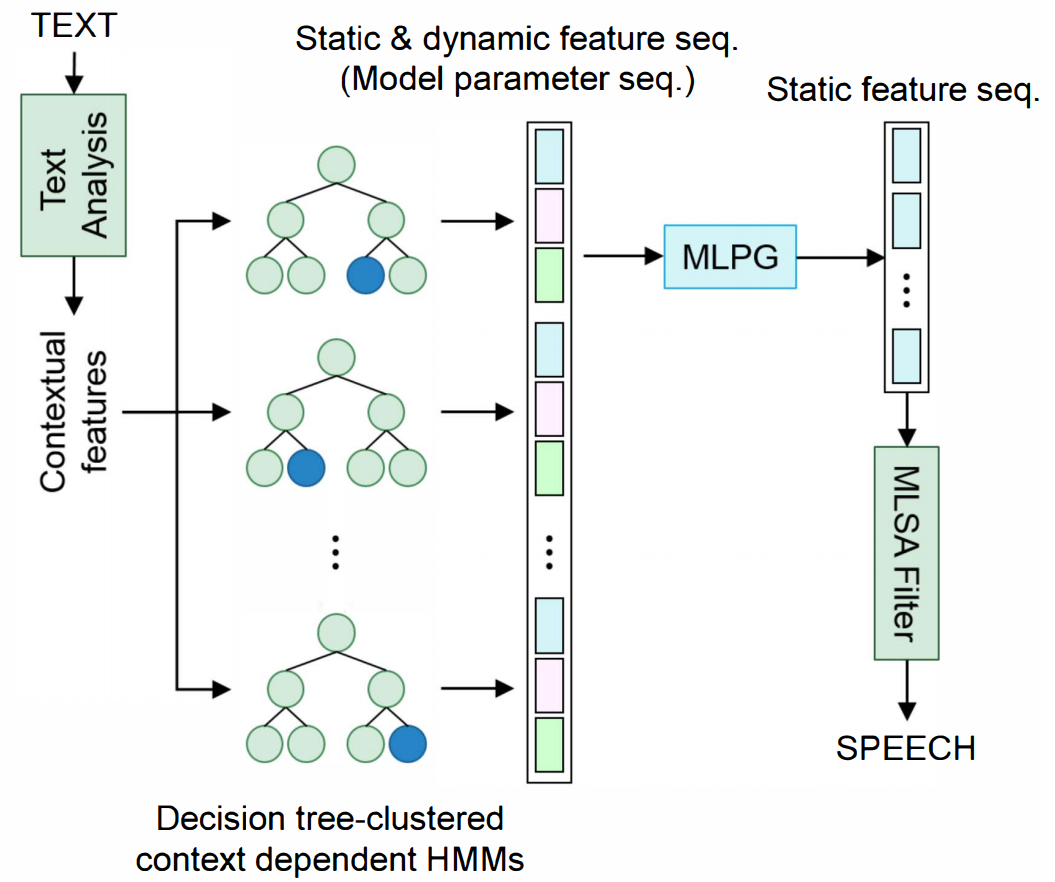
\includegraphics[width=\linewidth]{images/hmm_spss.png}
		\captionof{figure}{The general HMM-based TTS pipeline.}
		\label{hmm_spss_framework}
	\end{minipage}
	\hspace{.05\linewidth}
	\begin{minipage}{.45\linewidth}
		\centering
		\begin{tabular}{| l | c |}
			\hline
			Method & MOS \\
			\hline
			HMM+MLPG & 3.08 ($\pm$0.12) \\
			HMM+DNN & 2.86 ($\pm$0.12) \\
			\textbf{DNN+MLPG} & \textbf{3.53 ($\pm$0.12}) \\
			DNN+DNN & 3.17 ($\pm$0.12) \\
			\hline
		\end{tabular}
		\captionof{table}{MOS of the different methods explored in \citep{Hashimoto-2015}. The first line is the HMM-based framework. For the second and fourth line, the MLPG algorithm is replaced by a fully-connected neural network.}
		\label{hashimoto_results}
	\end{minipage}
\end{figure}

Improvements to this framework were later brought by feed-forward deep neural networks (DNN), as a result of progress in both hardware and software. \cite{SPSSDNN} proposes to replace entirely the decision tree-clustered HMMs in favor of a DNN. They argue for better data efficiency as the training set is no longer fragmented in different clusters of contexts. They demonstrate improvements over the speech quality with a number of parameters similar to that of the HMM-based approach. Later researches corroborate these findings \citep{OnTheTrainingAspects, Hashimoto-2015}. The MOS of different model combinations tried by \citep{Hashimoto-2015} are reported in Table \ref{hashimoto_results}

\citep{BDLSTMTTS} support that RNNs make natural acoustic models as they are able to learn a compact representation of complex and long-span functions. As RNNs are fit to generate temporally consistent series, the static features can directly be determined by the acoustic model, alleviating the need for dynamic features and MLPG. They compare networks of bidirectional LSTMs against the HMM and DNN based approaches described previously. Their A/B testing results are conclusive, we report them in figure \ref{dblstm_subjective}.

\begin{figure}[h]
	\centering
	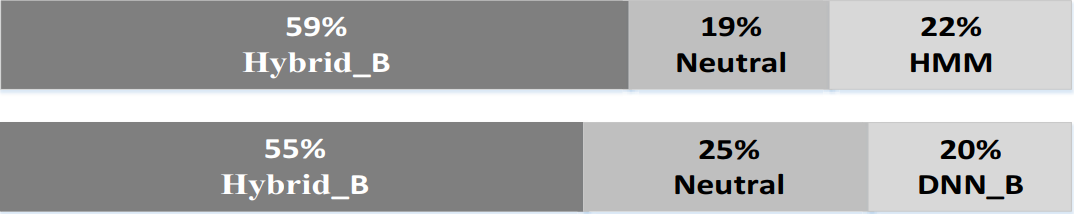
\includegraphics[width=0.6\linewidth]{images/bdlstm_subjective.png}
	\caption{A/B testing of the models. Hybrid\_B is a network with fully-connected and bidirectional LSTM layers.}
	\label{dblstm_subjective}
\end{figure}

The coming of WaveNet \citep{WaveNet} made a substantial breakthrough in TTS. WaveNet is a deep convolutional neural network that, for a raw audio waveform, models the distribution of a single sample given all previous ones. It is thus possible to directly generate audio by predicting samples one at a time in an autoregressive fashion. WaveNet leverages stacks of one-dimensional dilated convolutions with a dilation factor increasing exponentially with the layer depth, allowing for the very large receptive field and the strong nonlinearity needed to model raw audio. Conditioning the model on linguistic features is required to perform TTS. WaveNet acts thus both as an acoustic model and as a vocoder. Note that without the local conditioning, a trained WaveNet generates sound alike the training data but without structure or semantics (essentially babbling). 
The authors compare WaveNet to an older parametric approach and to a concatenative approach, the results are reported in Figure \ref{wavenet_results}. The parametric approach is an LSTM-based system while the other is an HMM-driven unit selection concatenative system (not detailed in this document). Notice how the results vary between US English and Mandarin Chinese, showing that TTS performance is not language agnostic.

\begin{figure}[h]
	\centering
	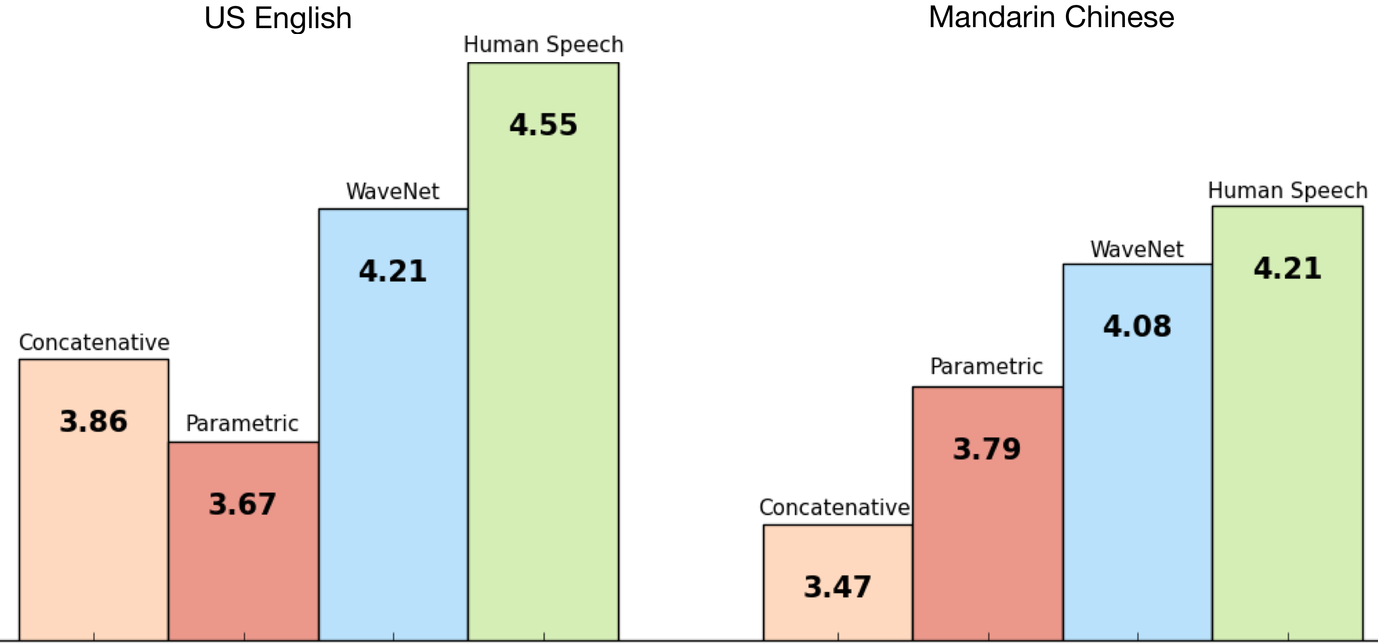
\includegraphics[width=.75\linewidth]{images/wavenet_results_chart.png}
	\caption{MOS of WaveNet's performance compared with a parametric and concatenative approach, as well as with natural speech.}
	\label{wavenet_results}
\end{figure}


%Deep Voice \citep{DeepVoice1} proposes a fully neural TTS framework that exploits WaveNet among other deep architectures. Deep Voice stands out by making use of only a few intermediate features: phonemes with stress annotations, phoneme durations,
%and F0. This has the advantage of making the framework easily transferable to new domains with little engineering effort as complex linguistic features need not be derived. The neural networks intervening in Deep Voice are: a grapheme-to-phoneme model that converts text to phonemes, a segmentation model that aligns a sequence of phonemes to an audio segment, a phoneme duration model that predicts the duration of each phoneme at generation time, a fundamental frequency model that predicts the V/UV flag with F0 values for voiced parts and finally, WaveNet which acts as an audio synthesis model. In all the works we presented previously, only the audio synthesis model was not manually engineered. While others have researched the use of neural networks for some of these components, Deep Voice is the first to simultaneously employ them all in a single framework. However, the grapheme-to-phoneme model is only used as a fallback for words not present in a phoneme dictionary. The roles and interactions of these components at training and inference time are shown in figure \ref{deep_voice_1_arch}. Deep Voice also improves on the inference time of WaveNet, with a speedup of up to 400. This allows for real-time or near real-time execution, with a tunable speed/quality trade-off. Deep Voice does not yield state of the art results but instead serves as groundwork for future researches. \color{red} discuss results \color{black}.
%
%\begin{figure}[h]
%	\centering
%	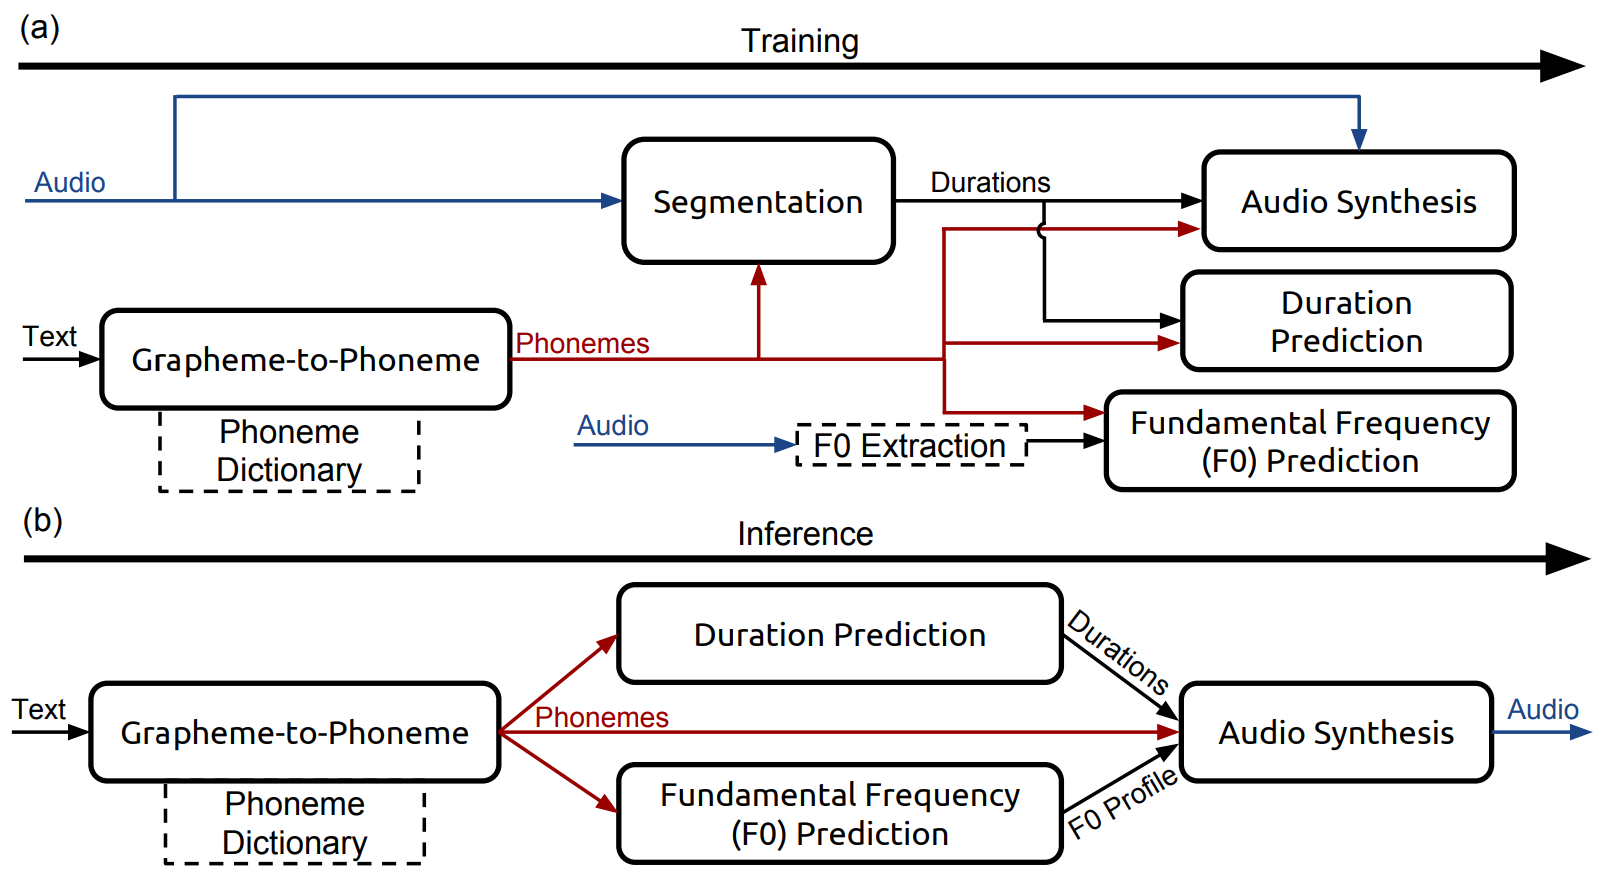
\includegraphics[width=.8\linewidth]{images/deep_voice_1_arch.png}
%	\caption{The training (a) and inference (b) procedure of Deep Voice. On the left of the image are the inputs, on the right are the outputs. Note that the segmentation model is only used for training.}
%	\label{deep_voice_1_arch}
%\end{figure}

% Up to 400x speedup on WaveNet
% Some previous research already use models to generate textual features
% No words with multiple pronunciations
% Natural MOS score when using ground truth F0 and durations
% Near real-time (accuracy/speed tradeoff)
% No diff when using original WaveNet

Follows Tacotron \citep{Tacotron1}, a sequence-to-sequence model that produces a spectrogram from a sequence of characters alone, further reducing the need for domain expertise. In this framework, the vocoder is the Griffin-Lim algorithm. Tacotron uses an encoder-decoder architecture where, at each step, the decoder operates on a weighted sum of the encoder outputs. This attention mechanism, described in \citep{Attention}, lets the network decide which steps of the input sequence are important with respect to each step of the output sequence. Tacotron achieves a MOS of 3.85 on a US English dataset, which is more than the 3.69 score obtained in the parametric approach of \citep{LSTM-RNN} but less than the 4.09 score obtained by the concatenative approach of \citep{ConcatenativeGoogle}. The authors mention that Tacotron is merely a step towards a better framework. Subsequently, Tacotron 2 is published \citep{Tacotron2}. The architecture of Tacotron 2 remains that of an encoder-decoder with attention although several changes to the type of layers are made. The main difference with Tacotron is the use of a modified WaveNet as vocoder. On the same dataset, Tacotron 2 achieves a MOS of 4.53, which compares to the 4.58 for human speech (the difference is not statistically significant), achieving the all-time highest MOS for TTS. With A/B testing, Tacotron 2 was found to be only slightly less preferred on average than ground truth samples. These ratings are shown in figure \ref{tacotron2_results}.

\begin{figure}[h]
	\centering
	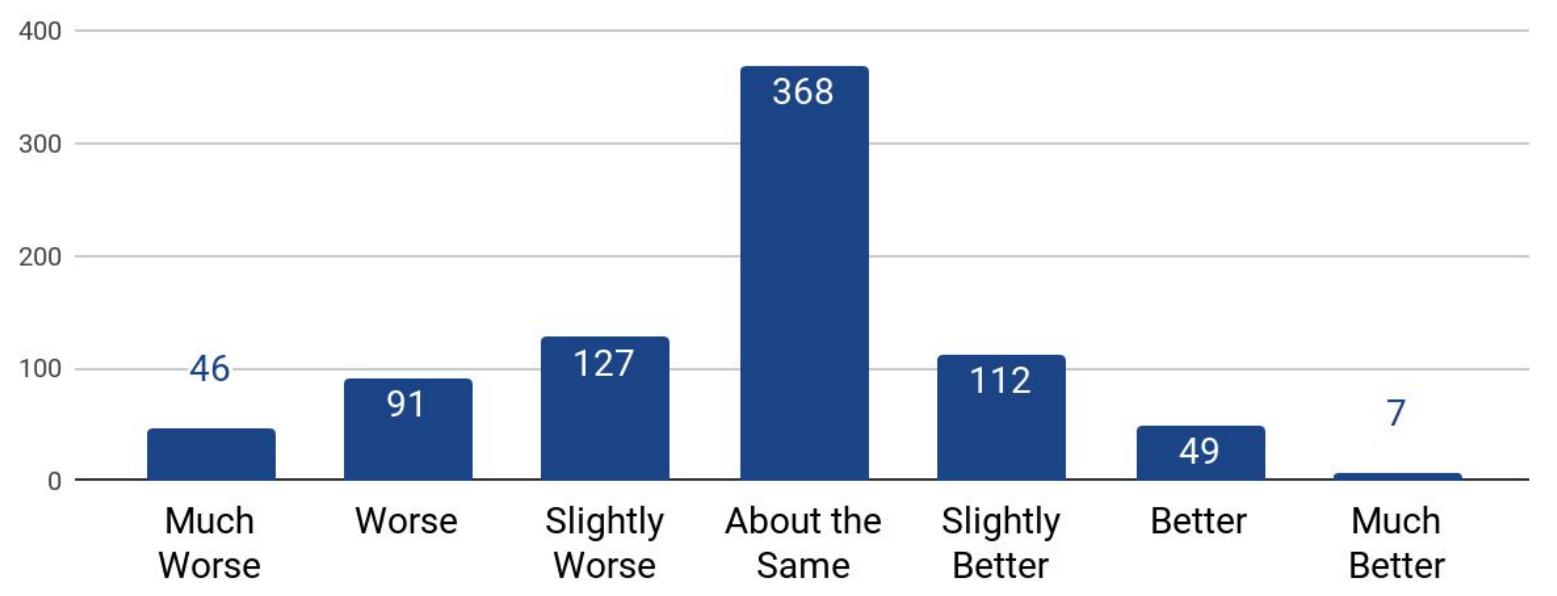
\includegraphics[width=.8\linewidth]{images/tacotron2_results.png}
	\caption{Preference ratings between Tacotron 2 and ground truth samples. There are 800 ratings from 100 items. The labels are expressed with respect to Tacotron 2.}
	\label{tacotron2_results}
\end{figure}

\color{red} Efficient neural audio synthesis? \color{black}

\section{Related voice cloning methods}


% Wavenet:
%The output is a categorical distribution over sample values. For tractability reasons, the output signal is restricted to 256 discrete values that correspond to a $\mu$-law quantization, which is invertible. The MOS resulting from one of the experiments suggests that there is no statistically significant degradation in the naturalness of speech quantized in this manner. The architecture of WaveNet comes with several non-trivial components, described in later sections of this document \color{red}link to the section\color{black}. 
% The audio generated by WaveNet requires no post-processing other than the inversion of the $\mu$-law. 
%Furthermore, it allows for conditioning with respect to a vector constant at every timestep (global conditioning), which can be used to designate the speaker identity. The authors suggest that WaveNet is able to encode the embedding of several speakers seen in training with a shared internal representation. Speaker identities are given as a one-hot encoding. 

\section{Transfer Learning from Speaker Verification to Multispeaker Text-To-Speech Synthesis}
\subsection{Overview}
Our solution to real-time voice cloning is largely based on \citep{SV2TTS} (referred to as SV2TTS throughout this document). It describes an approach to zero-shot voice cloning that only requires 5 seconds of reference speech. This paper is only one of the many publications from the Tacotron series\footnote{\url{https://google.github.io/tacotron/}} authored at Google. Interestingly, the SV2TTS paper does not bring much innovation of its own, rather it is based on three major earlier works from Google: the GE2E loss \citep{GE2E}, Tacotron \citep{Tacotron1} and WaveNet \citep{WaveNet}. The complete framework is a three-stage pipeline, where the steps correspond to the models listed in order previously. Many of the current TTS tools and functionalities provided by Google, such as the Google assistant\footnote{\url{https://assistant.google.com/}} or the Google cloud services\footnote{\url{https://cloud.google.com/text-to-speech/}}, make use of these same models. While there are many open-source reimplementations of these models online, there is none of the SV2TTS framework to our knowledge (as of May 2019).

The three stages of the framework are as follows:
\begin{itemize}
	\item A speaker encoder that derives an embedding from the short utterance of a single speaker. The embedding is a meaningful representation of the voice of the speaker, such that similar voices are close in latent space. This model is described in \citep{GE2E} (referred as GE2E throughout this document) and \citep{TE2E}.
	\item A synthesizer that, conditioned on the embedding of a speaker, generates a spectrogram from a text. This model is the popular Tacotron 2 \citep{Tacotron2} without WaveNet (which is often referred to as just Tacotron because it is largely similar to the first iteration).
	\item A vocoder that infers an audio waveform from the spectrograms generated by the synthesizer. The authors used WaveNet \citep{WaveNet} as a vocoder, effectively reapplying the entire Tacotron 2 framework.
\end{itemize}
At inference time, the speaker encoder is fed a short reference utterance of the speaker to clone. It generates an embedding that is used to condition the synthesizer, and a text processed as a phoneme sequence is given as input to the synthesizer. The vocoder takes the output of the synthesizer to generate the speech waveform. This is illustrated in figure \ref{sv2tts_framework}.

\begin{figure}[h]
	\centering
	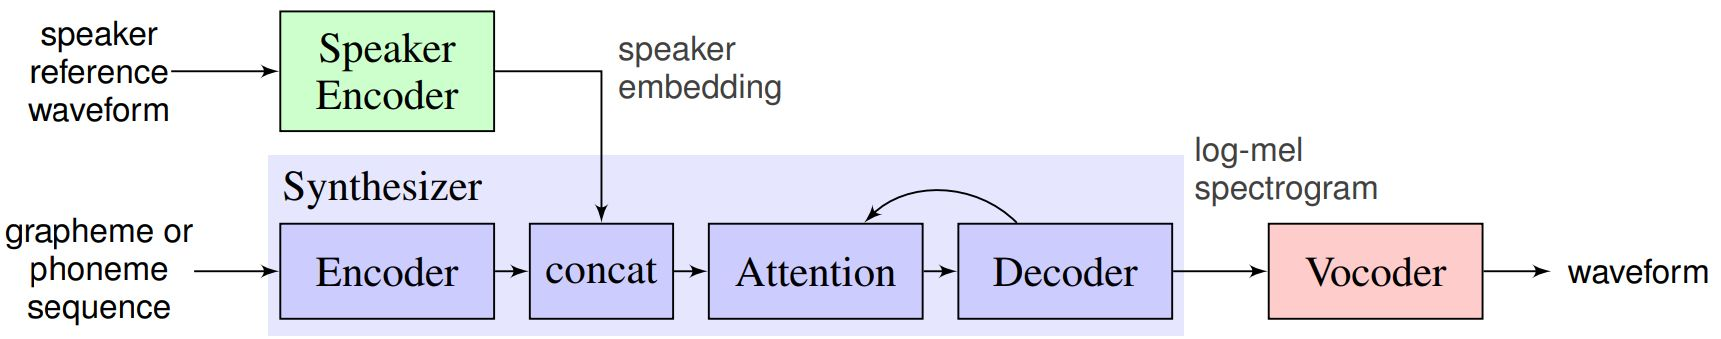
\includegraphics[width=\linewidth]{images/sv2tts_framework.jpg}
	\caption{The SV2TTS framework. The blue blocks represent a high-level view of the Tacotron architecture modified to allow conditioning.}
	\label{sv2tts_framework}
\end{figure}

A particularity of the SV2TTS framework is that all models can be trained separately and on distinct datasets. For the encoder, one seeks to have a model that is robust to noise and able to capture the many characteristics of the human voice. Therefore, a large corpus of many different speakers would be preferable to train the encoder, without any strong requirement on the noise level of the audios. Additionally, the encoder is trained with the GE2E loss which requires no labels other than the speaker identity. With GE2E, the task to be learned by the model is a speaker verification task, which by itself has little to do with voice cloning. However, the task is stipulated in way that the network will output an embedding that is a meaningful representation of the voice of the speaker. This embedding is suitable for conditioning the synthesizer on a voice, hence the name of the paper: "Transfer Learning from Speaker Verification to Multispeaker Text-To-Speech Synthesis". For the datasets of the synthesizer and the vocoder, transcripts are required and the quality of the generated audio can only be as good as that of the data. Higher quality and annotated datasets are thus required, which often means they are smaller in size.

In subsection \ref{problem_definition}, we formally define the task that SV2TTS aims to solve. In the remaining subsections, we present the three parts of the framework as described in \citep{SV2TTS}.


\subsection{Problem definition} \label{problem_definition}
\newcommand{\vx}{\mathbf{x}}
\newcommand{\vu}{\mathbf{u}}
\newcommand{\ve}{\mathbf{e}}
\newcommand{\vt}{\mathbf{t}}
\newcommand{\vc}{\mathbf{c}}
\newcommand{\vw}{\mathbf{w}}
\newcommand{\ms}{\mathbf{S}}
\newcommand{\enc}{\mathcal{E}}
\newcommand{\syn}{\mathcal{S}}
\newcommand{\voc}{\mathcal{V}}
Consider a dataset of utterances grouped by their speaker. We denote the $j$th utterance of the $i$th speaker as $\vu_{ij}$. Utterances are in the waveform domain. We denote by $\vx_{ij}$ the log-mel spectrogram of the utterance $\vu_{ij}$. A log-mel spectrogram is a deterministic, non-invertible (lossy) but derivable function that extracts speech features from a waveform, so as to handle audio in a more tractable fashion in machine learning.

The encoder $\enc$ computes the embedding $\ve_{ij} = \enc(\vx_{ij}; \vw_\enc)$ corresponding to the utterance $\vu_{ij}$, where $\vw_\enc$ are the parameters of the encoder. %Note that we haven't defined the optimization objective of this model yet.

The synthesizer $\syn$, parametrized by $\vw_\syn$, is tasked to approximate $\vx_{ij}$ given $\ve_{ij}$ and $\vt_{ij}$, the transcript of utterance $\vu_{ij}$. We have $\hat\vx_{ij} = \syn(\ve_{ij}, \vt_{ij}; \vw_\syn)$.

Finally, the vocoder $\voc$, parametrized by $\vw_\voc$, is tasked to approximate $\vu_{ij}$ given $\hat\vx_{ij}$. We have $\hat\vu_{ij} = \voc(\hat\vx_{ij}; \vw_\voc)$.

One could train this framework in an end-to-end fashion with the following objective function:
$$ min_{\vw_\enc, \vw_\syn, \vw_\voc} L_\voc(\vu_{ij}, \voc(\syn(\enc(\vx_{ij}; \vw_\enc), \vt_{ij}; \vw_\syn); \vw_\voc)) $$
Where $L_\voc$ is a loss function in the waveform domain. This approach has drawbacks:
\begin{itemize}
	\item It requires training all three models on a same dataset, meaning that this dataset would ideally need to meet the requirements for all models: large number of speakers for the encoder but at the same time transcripts for the synthesizer and low level noise for the synthesizer and somehow an average noise level for the encoder (so as to be able to handle noisy input speech). These conflicts are problematic and would lead to training models that could perform better if trained separately on distinct datasets. Specifically, a small dataset will likely lead to poor generalization and thus poor zero-shot performance.
	\item The convergence of the combined model could be very hard to reach. In particular, the Tacotron synthesizer typically takes a significant time before producing correct alignments (see \rw).
\end{itemize}

An evident way of making the problem easier is to separate the training of the synthesizer and of the vocoder. Assuming a pretrained encoder, the synthesizer can be trained directly on the mel spectrograms of the target audio:
$$ min_{\vw_\syn} L_\syn(\vx_{ij}, \syn(\ve_{ij}, \vt_{ij}; \vw_\syn)) $$
Where $L_\syn$ is a loss function in the time-frequency domain. 

The vocoder is then trained directly on the spectrograms. Note that both the approaches of training on ground truth spectrograms or on synthesizer-generated spectrograms are valid (see \rw). The latter requires a pretrained synthesizer.
$$ min_{\vw_\voc} L_\voc(\vu_{ij}, \voc(\vx_{ij}; \vw_\voc)) \ \ \text{or} \ \ 
   min_{\vw_\voc} L_\voc(\vu_{ij}, \voc(\hat\vx_{ij}; \vw_\voc))$$

Remains the optimization of the speaker encoder. Unlike the synthesizer and the vocoder, the encoder does not have labels to be trained on. The task is lousily defined as producing "meaningful" embeddings that characterize the voice in the utterance. One could conceive of a way to train the speaker encoder as an autoencoder, but it would require the corresponding upsampling model to be made aware of the text to predict. Either the dataset is constrained to a same sentence, either one needs transcripts and the upsampling model is the synthesizer. In both cases the quality of the training is impaired by the dataset and unlikely to generalize well.

Fortunately, the GE2E loss \citep{GE2E} brings a solution to this problem and allows to train the speaker encoder independently of the synthesizer


- what it means for each network to generalize


%\section{Speed}
%Note that all models are interchangeable provided that they perform the same task. In particular, vanilla WaveNet is extremely slow for inference. Several later papers brought improvements on that aspect to bring the generation near real-time or faster than real-time, e.g. \citep{ParallelWaveNet}, \citep{FastWaveNet}. Note that in this context, real-time is achieved when the generation time is shorter than or equal to the duration of the generated audio. In our implementation, the vocoder used is based on WaveRNN \citep{WaveRNN}.







\clearpage
\bibliographystyle{plainnat}
\bibliography{references} 




















%$$\Leftrightarrow h_b(x) =
%\left\{\begin{array}{lll}
%0 & if & P(y = 0 | x) > P(y = 1 | x)\\ 
%1 & else &
%\end{array}\right.$$



%\begin{figure}[h]
%	\centering
%	\includegraphics[width=16cm]{image.png}
%	\caption{caption}
%	\label{label}
%\end{figure}



%\begin{figure}[h]
%	\centering
%	\captionsetup{justification=centering}
%	\hspace{-1cm}
%	\subfigure{\includegraphics[height=5cm]{image.png}}
%	\subfigure{\includegraphics[height=5cm]{image.png}}
%	\hspace{-1cm}
%	\caption{caption}
%	\label{label}
%\end{figure}


%\begin{center}
%	\begin{tabular}{|r|ccc|ccc|}
%		\hline
%		& \multicolumn{6}{c|}{Validation set}\\
%		\hline
%		& \multicolumn{3}{c|}{Valid images (3126)} & \multicolumn{3}{c|}{Invalid images (3126)} \\
%		\hline
%		& Correct & Unclassified & Incorrect & Correct & Unclassified & Incorrect \\
%		\hline
%		Reduced & 94.98\% & 3.07\% & 1.95\% & 95.27\% & 2.91\% & 1.82\% \\
%		Lenet & 98.08\% & 0.74\% & 1.18\% & 97.86\% & 0.96\% & 1.18\% \\
%		\hline
%	\end{tabular}
%	
%	\vspace{0.5cm}
%	  
%	\begin{tabular}{|r|ccc|ccc|}
%		\hline
%		& \multicolumn{6}{c|}{Test set}\\
%		\hline
%		& \multicolumn{3}{c|}{Valid images (999)} & \multicolumn{3}{c|}{Invalid images (74)} \\
%		\hline
%		& Correct & Unclassified & Incorrect & Correct & Unclassified & Incorrect \\
%		\hline
%		Reduced& 94.29\% & 3.70\% & 2.00\% & 95.95\% & 4.05\% & 0.00\%  \\
%		Lenet & 96.90\% & 1.30\% & 1.80\% & 97.30\% & 1.35\% & 1.35\% \\
%		\hline
%	\end{tabular}
%\end{center}


\end{document}













































































































